\documentclass{article}
\usepackage[utf8]{inputenc}
\usepackage{graphicx}
\usepackage{xcolor}
\definecolor{mydarkgray}{RGB}{55, 55, 55}
\definecolor{mydarkviolet}{RGB}{102, 0, 153}
\usepackage[hidelinks, colorlinks=true, linkcolor=mydarkviolet, urlcolor=mydarkviolet, citecolor=cyan]{hyperref}
\usepackage{listings}
\usepackage{ragged2e}  
\usepackage{float}
\usepackage{url} 
\usepackage{animate}

\title{\Huge \textbf{Práctica 7: Sistema de Observación Meteorológica usando el Patron Observador}}
\author{
  Jorge Domínguez González (\href{mailto:alu0101330600@ull.edu.es}{alu0101330600@ull.edu.es}) \and
  Adnan (\href{mailto:Alu01@ull.edu.es}{alu01@ull.edu.es}) \and
  Paula (\href{mailto:alu01@ull.edu.es}{alu01@ull.edu.es})
}
\date{\today}

\begin{document}
\maketitle

\tableofcontents
\listoffigures
\newpage

\section{Introducción}
El código proporcionado presenta una implementación de un sistema de observación meteorológica en Java. Este sistema utiliza el patrón de diseño Observador para recibir actualizaciones de las condiciones meteorológicas de diversas ciudades a través de la API de WeatherStack.

\section{Estructura del Código}

\subsection{Clase \texttt{WeatherStackAPI}}
La clase \texttt{WeatherStackAPI} se encarga de interactuar con la API de WeatherStack para obtener las condiciones meteorológicas de una ciudad específica. Utiliza la biblioteca Unirest para realizar solicitudes HTTP.

\begin{itemize}
    \item \textbf{Método \texttt{getWeatherConditionsFrom(String zone)}}: Este método recibe el nombre de una ciudad como parámetro, realiza una solicitud a la API de WeatherStack y devuelve las condiciones meteorológicas en formato JSON.
\end{itemize}

\begin{figure}[H]
    \centering
    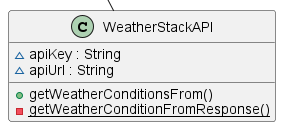
\includegraphics[width=0.4\textwidth]{weatherstack.png}
    \caption{Diagrama de Clase weatherstack}
    \label{figura:weatherstack}
\end{figure}

\subsection{Interfaz \texttt{Observador}}
La interfaz \texttt{Observador} define el método \texttt{actualizar}, que las clases interesadas en recibir actualizaciones meteorológicas deben implementar.
\begin{figure}[H]
    \centering
    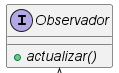
\includegraphics[width=0.4\textwidth]{IObservador.png}
    \caption{Diagrama de Clase IObservador}
    \label{figura:IObservador}
\end{figure}

\subsection{Clase \texttt{PantallaMeteorologica}}
La clase \texttt{PantallaMeteorologica} implementa la interfaz \texttt{Observador} y representa la interfaz gráfica que mostrará las condiciones meteorológicas. Utiliza la biblioteca Swing para la interfaz de usuario.

\begin{itemize}
    \item \textbf{Método \texttt{actualizar(String condiciones)}}: Este método recibe las condiciones meteorológicas como una cadena JSON y actualiza la interfaz gráfica con la información relevante.
\end{itemize}

\begin{figure}[H]
    \centering
    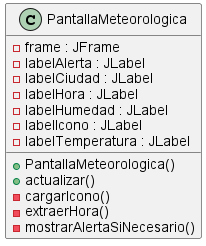
\includegraphics[width=0.4\textwidth]{PantallaMeteo.png}
    \caption{Diagrama de Clase PantallaMeteo}
    \label{figura:PantallaMeteo}
\end{figure}

\subsection{Clase \texttt{SeleccionCiudad}}
La clase \texttt{SeleccionCiudad} se encarga de permitir al usuario seleccionar las ciudades para las cuales desea recibir actualizaciones meteorológicas. Utiliza la biblioteca Swing para la interfaz de usuario.
\begin{figure}[H]
    \centering
    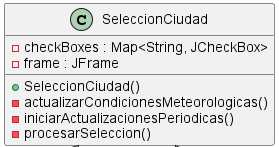
\includegraphics[width=0.4\textwidth]{seleccionCiudad.png}
    \caption{Diagrama de Clase seleccionCiudad}
    \label{figura:seleccionCiudad}
\end{figure}
\subsection{Clase \texttt{SujetoWeatherstack}}
La clase \texttt{SujetoWeatherstack} actúa como el sujeto que mantiene una lista de observadores interesados en recibir actualizaciones meteorológicas.

\begin{itemize}
    \item \textbf{Método \texttt{agregarObservador(Observador observador)}}: Este método agrega un observador a la lista de observadores.
    \item \textbf{Método \texttt{notificarObservadores(String condiciones)}}: Este método notifica a todos los observadores registrados con las condiciones meteorológicas actualizadas.
\end{itemize}

\begin{figure}[H]
    \centering
    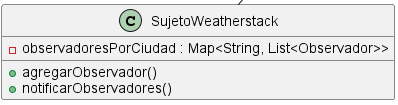
\includegraphics[width=0.4\textwidth]{weatherstacksujeto.png.png}
    \caption{Diagrama de Clase weatherstacksujeto.png}
    \label{figura:weatherstacksujeto.png}
\end{figure}
\subsection{Método \texttt{main}}
El método \texttt{main} se encuentra en la clase \texttt{MainWeatherstack} y sirve como punto de entrada para la aplicación.

\begin{itemize}
    \item Configura la interfaz de usuario inicializando instancias de \texttt{PantallaMeteorologica} y \texttt{SeleccionCiudad}.
    \item Registra la instancia de \texttt{PantallaMeteorologica} como observador en la instancia de \texttt{SujetoWeatherstack}.
    \item Permite al usuario seleccionar ciudades y muestra las condiciones meteorológicas en la interfaz gráfica.
\end{itemize}

\section{Pasos del Flujo del Programa}
El programa sigue estos pasos:

\begin{enumerate}
    \item Se inicia la aplicación desde el método \texttt{main}.
    \item Se configuran las instancias de la interfaz de usuario y se registran los observadores.
    \item El usuario selecciona las ciudades de interés.
    \item Se realiza una solicitud a la API de WeatherStack para obtener las condiciones meteorológicas de las ciudades seleccionadas.
    \item Las condiciones meteorológicas se notifican a los observadores (instancia de \texttt{PantallaMeteorologica}) que actualizan la interfaz gráfica.
    \item El proceso se repite cuando el usuario selecciona nuevas ciudades.
\end{enumerate}

\section{Interfaz Gráfica para el Usuario}
La interfaz gráfica incluye una pantalla para mostrar las condiciones meteorológicas y un formulario para que el usuario seleccione las ciudades de interés.

\begin{figure}[H]
    \centering
    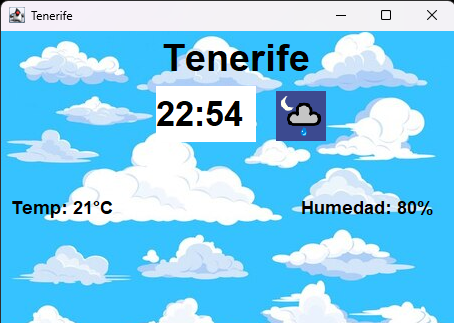
\includegraphics[width=0.7\textwidth]{Pantalla.png}
    \caption{Interfaz de Pantalla Meteorológica}
    \label{fig:pantalla_meteorologica}
\end{figure}

\begin{figure}[H]
    \centering
    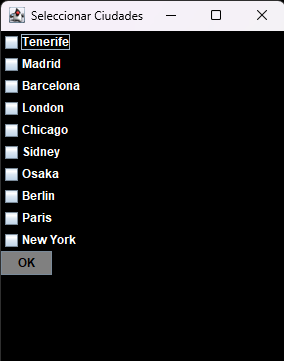
\includegraphics[width=0.5\textwidth]{Seleccion_ciudades.png}
    \caption{Interfaz de Selección de Ciudad}
    \label{fig:seleccion_ciudad}
\end{figure}

\section{Diagrama UML}
El diagrama de clases UML muestra las relaciones entre las clases del sistema.

\begin{figure}[H]
    \centering
    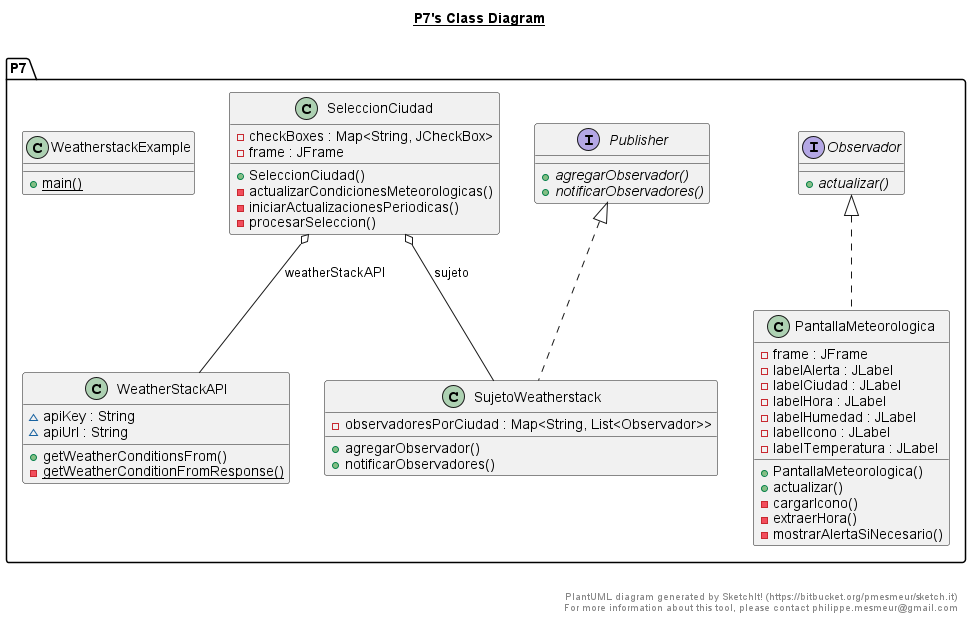
\includegraphics[width=0.7\textwidth]{Diagrama_clases.png}
    \caption{Diagrama de Clases UML}
    \label{fig:diagrama_clases}
\end{figure}

\section{Estimación de Plazo}
Se estima que el desarrollo del proyecto tomará aproximadamente el siguiente tiempo:

\begin{table}[H]
    \centering
    \begin{tabular}{|l|c|c|}
        \hline
        \textbf{TAREA} & \textbf{TIEMPO ESPERADO} & \textbf{TIEMPO FINAL} \\
        \hline
        Implementación del Sistema & 4 Horas & 8 Horas \\
        Pruebas y Depuración & 4 Horas & 4 Horas \\
        Documentación & 2 Horas & 3 Horas \\
        Implementación en GitHub & 1 Hora & 2 Horas \\
        \hline
    \end{tabular}
    \caption{Estimación de Plazo}
    \label{tab:estimacion_plazo}
\end{table}

\section{Conclusiones}
El sistema de observación meteorológica implementado proporciona una interfaz amigable para que los usuarios obtengan información en tiempo real sobre las condiciones meteorológicas de las ciudades de su elección. El uso del patrón Observador facilita la actualización automática de la interfaz de usuario cuando cambian las condiciones meteorológicas.

\section{Bibliografía}
\begin{thebibliography}{99}
    \bibitem{weatherstack-api-docs}
    Documentación de la API de WeatherStack. \url{https://weatherstack.com/documentation}

    \bibitem{unirest-docs}
    Documentación de Unirest. \url{http://kong.github.io/unirest-java/}
\end{thebibliography}

\end{document}